\documentclass[addpoints,10pt]{exam}
\usepackage{amsmath, amssymb}
\usepackage{ifthen}
\usepackage{graphicx}
\usepackage[top=0.6in, left=0.6in, right=0.6in, bottom=0.6in]{geometry}


%%%%%%%%%%%%%%%%%%%%%%%%%%%%%%%%%%%%%%%
%-------------SHOWTO COMMAND-------------
%%%%%%%%%%%%%%%%%%%%%%%%%%%%%%%%%%%%%%%

%This is a convenience command for conditional compilation that controls which questions are shown to a particular recitation section on the quiz. Any question not enclosed by \showto is shown to all recitation sections. The first argument to \showto is the desired section number. The second argument is the question body
\newcommand{\showto}[2]
{
\ifthenelse{
	 \equal{\RecitationSection}{#1}\OR\equal{\RecitationSection}{MASTER}
	}{#2}{}
}
%%%%%%%%%%%%%%%%%%%%%%%%%%%%%%%%%%%%%%%
%-----------END SHOWTO COMMAND------------
%%%%%%%%%%%%%%%%%%%%%%%%%%%%%%%%%%%%%%%



%%%%%%%%%%%%%%%%%%%%%%%%%%%%%%%%%%%%%%%
%------------------OPTIONS------------------
%%%%%%%%%%%%%%%%%%%%%%%%%%%%%%%%%%%%%%%
%\boxedpoints
%\pointsinmargin

%Show or hide answers
\printanswers
%\noprintanswers
%%%%%%%%%%%%%%%%%%%%%%%%%%%%%%%%%%%%%%%
%---------------END OPTIONS-----------------
%%%%%%%%%%%%%%%%%%%%%%%%%%%%%%%%%%%%%%%





%%%%%%%%%%%%%%%%%%%%%%%%%%%%%%%%%%%%%%%
%------------ SELECT SECTION-----------------
%%%%%%%%%%%%%%%%%%%%%%%%%%%%%%%%%%%%%%%

%To switch between different versions of the quiz for different recitation sections, change the final argument as needed to 201, 202, 203, 204, etc. If you instead enter MASTER you'll get a document with all quiz questions.
\newcommand{\RecitationSection}{MASTER}

%%%%%%%%%%%%%%%%%%%%%%%%%%%%%%%%%%%%%%%
%------------END SELECT SECTION--------------
%%%%%%%%%%%%%%%%%%%%%%%%%%%%%%%%%%%%%%%





%%%%%%%%%%%%%%%%%%%%%%%%%%%%%%%%%%%%%%%
%---------------QUIZ HEADER-----------------
%%%%%%%%%%%%%%%%%%%%%%%%%%%%%%%%%%%%%%%
\begin{document}
\thispagestyle{empty}

\noindent \textbf{Econ 103 --  Quiz 1}

\vspace{15pt}
\noindent
\makebox[0.45\textwidth]{Name:\enspace\hrulefill}

\paragraph{Instructions: } This is closed-book, closed-notes quiz. Please write your answers in the blanks provided. Each question is worth one point but no partial credit will be awarded. Non-programmable calculators are permitted.

\vspace{5pt}
%%%%%%%%%%%%%%%%%%%%%%%%%%%%%%%%%%%%%%%
%-------------END QUIZ HEADER----------------
%%%%%%%%%%%%%%%%%%%%%%%%%%%%%%%%%%%%%%%

\setlength\answerlinelength{2in}

\begin{questions}

%QUESTION 1
%%%%%%%%%%%%%%%%
\showto{201}{\question To find out if smoking causes lower grades, Sara asks 100 of her friends if they smoke and what their current GPA is. Has Sara collected observational or experimental data? \answerline[]}





%QUESTION 2

%%%%%%%%%%%%%%%%%%%%%%%
\showto{203}{\question Assume we collect data on handspan in centimeters of students in ECON 103. What units does the \emph{median} of handspan have? \answerline[]}

\showto{205}{\question Assume we collect data on handspan in centimeters of students in ECON 103. What units does the \emph{variance} of handspan have? \answerline[]}



%%%%%%%%%%%%%%%%%%%%%%%

% QUESTION 3

%%%%%%%%%%%%%%%%%%%%%%%

\showto{205}{\question What is the expression $\displaystyle \sqrt{\frac{1}{n-1} \sum_{i=1}^n (x_i - \bar{x})^2}$ the definition of? \answerline[]}


\showto{202}{\question Write down the formula for the sample mean and the sample skewness, in terms of individual observations, $x_1, x_2 \hdots x_n$.  \answerline[]} 

\vspace{0.5in}

%%%%%%%%%%%%%%%%%%%%%%%

% QUESTION 4

%%%%%%%%%%%%%%%%%%%%%%%

\showto{204}{\question I have a dataset in which, strangely enough, every observation equals 7. What is the interquartile range of this dataset? \answerline[]}



% QUESTION 5

%%%%%%%%%%%%%%%%%%%%%%%


\showto{203}{\question I have a dataset for which the mean is $3$. If I add 1 to each number in the dataset, what is the new mean? \answerline[]}

\showto{202}{\question I have a dataset for which the standard deviation is $3$. If I add 1 to each number in the dataset, what is the new standard deviation? \answerline[]}

%%%%%%%%%%%%%%%%%%%%%%%

% QUESTIONS 6, 7, 8

%%%%%%%%%%%%%%%%%%%%%%%
{\question The sample mean is a measure of what? \\
\begin{oneparchoices}
	\choice Symmetry
	\choice Spread
	\choice Central Tendency
\end{oneparchoices}\answerline}

{\question The variance is a measure of what? \\
\begin{oneparchoices}
	\choice Symmetry
	\choice Spread
	\choice Central Tendency
\end{oneparchoices}\answerline}

{\question Skewness is a measure of what? \\
\begin{oneparchoices}
	\choice Symmetry
	\choice Spread
	\choice Central Tendency
\end{oneparchoices}\answerline}

%%%%%%%%%%%%%%%%%%%%%%%

% QUESTION 9

%%%%%%%%%%%%%%%%%%%%%%%
\showto{204}{\question What is the result of the following sequence of R commands? (Hint: R will print a single word (a logical statement) after the fourth line - write down this word)   \answerline[]
\texttt{x <- 5\\
    y <- 7\\
    z = x + y\\
    z + 3 == 15}}



%%%%%%%%%%%%%%%%%%%%%%%
%For each of the variables, indicate whether it is nominal, ordinal or numerical
{\question Indicate whether this variable is nominal, ordinal or numerical: Ratings of movies (very poor, poor, average, good, very good)  \answerline[]}

{\question Indicate whether this variable is nominal, ordinal or numerical: Means of transportation (walking, bus, train, car)  \answerline[]}

{\question Indicate whether this variable is nominal, ordinal or numerical: Monthly income (in US dollars)  \answerline[]}



%%%%%%%%%%%%%%%
% % % Question 5
\showto{201}{
\question Is the skewness of this distribution positive, negative or zero?
\begin{figure}[ht!]
\begin{center}
%\caption{Desired and actual maintenance of community \textsl{i}}
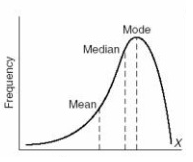
\includegraphics[scale=1]{NegSkew.png}
\end{center}
\end{figure}
\answerline[]
}

%%%%%%%%%%%%%%%% Question 4
%%%%%%%%%%%%%%%%%%%%%%%
\showto{201}{\question What is the sample mean and variance of the z-scores $z_1, z_2,\hdots, z_n$? \answerline[]}

%%%%%%%%%%%%%%%
\showto{201}{\question In the following diagram, events $A$, $B$, $C$, $D$ and $E$ are mutually exclusive and collectively exhaustive. True or false?  \answerline[]
%\begin{figure}[ht!]
%\begin{center}
%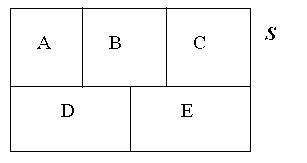
\includegraphics[scale=1]{figure1}
%\end{center}
%\end{figure}
}


\showto{205}{
	\question Out of a sample of 300 students, the undergraduate group in economics needs to chose three students for a committee: one president, one vice-president and one treasurer. Write down an expression for the total possible number of different committees (you do not have to actually calculate the probability).
	\answerline[]
}

\showto{205}{\question Two six sided fair dice (with numbers 1 to 6) are rolled. What is the probability \textbf{in fraction} that their sum is (strictly) greater 9?
	\answerline[]}


\end{questions}

\end{document}  